% Autómata Finito Determinista del Analizador Léxico de MiniJava - Etapa 1
% Fuente: src/main/java/analizadorlexico/AnalizadorLexico.java (un estado = un método)
% Compilar con:  pdflatex AutomataLexico.tex
%
% Convenciones (resumen):
%  - Doble círculo = estado final: ante un carácter sin transición propia emite
%    su token y vuelve a e0 SIN consumir ese carácter (queda como adelanto).
%  - Flecha punteada roja = error léxico (ExcepcionLexica, fin del análisis).
%  - EOF actúa como "otro" en los estados finales y como error en string,
%    caracter y comentario de bloque.
%  - idMV devuelve pr_<palabra> si el lexema es una palabra reservada.
%  - simple = op* op% ( ) { } [ ] ; , . :  (el token lo indica la etiqueta).
%  - ERROR aparece dibujado dos veces (norte y sur) por legibilidad: es un
%    único estado.
\documentclass{article}
\usepackage[paperwidth=23.5cm,paperheight=22.5cm,margin=6mm]{geometry}
\usepackage[utf8]{inputenc}
\usepackage{tikz}
\usetikzlibrary{automata,positioning,arrows}
\pagestyle{empty}

\tikzset{
  >=stealth',
  every state/.style={minimum size=7.5mm, inner sep=1pt, font=\footnotesize\ttfamily},
  every edge/.style={draw, ->},
  lab/.style={font=\scriptsize\ttfamily, inner sep=1.5pt},
  lg/.style={font=\scriptsize, inner sep=1.5pt},
  err/.style={dashed, draw=red!70!black, text=red!70!black}
}

\begin{document}
\noindent
\begin{center}
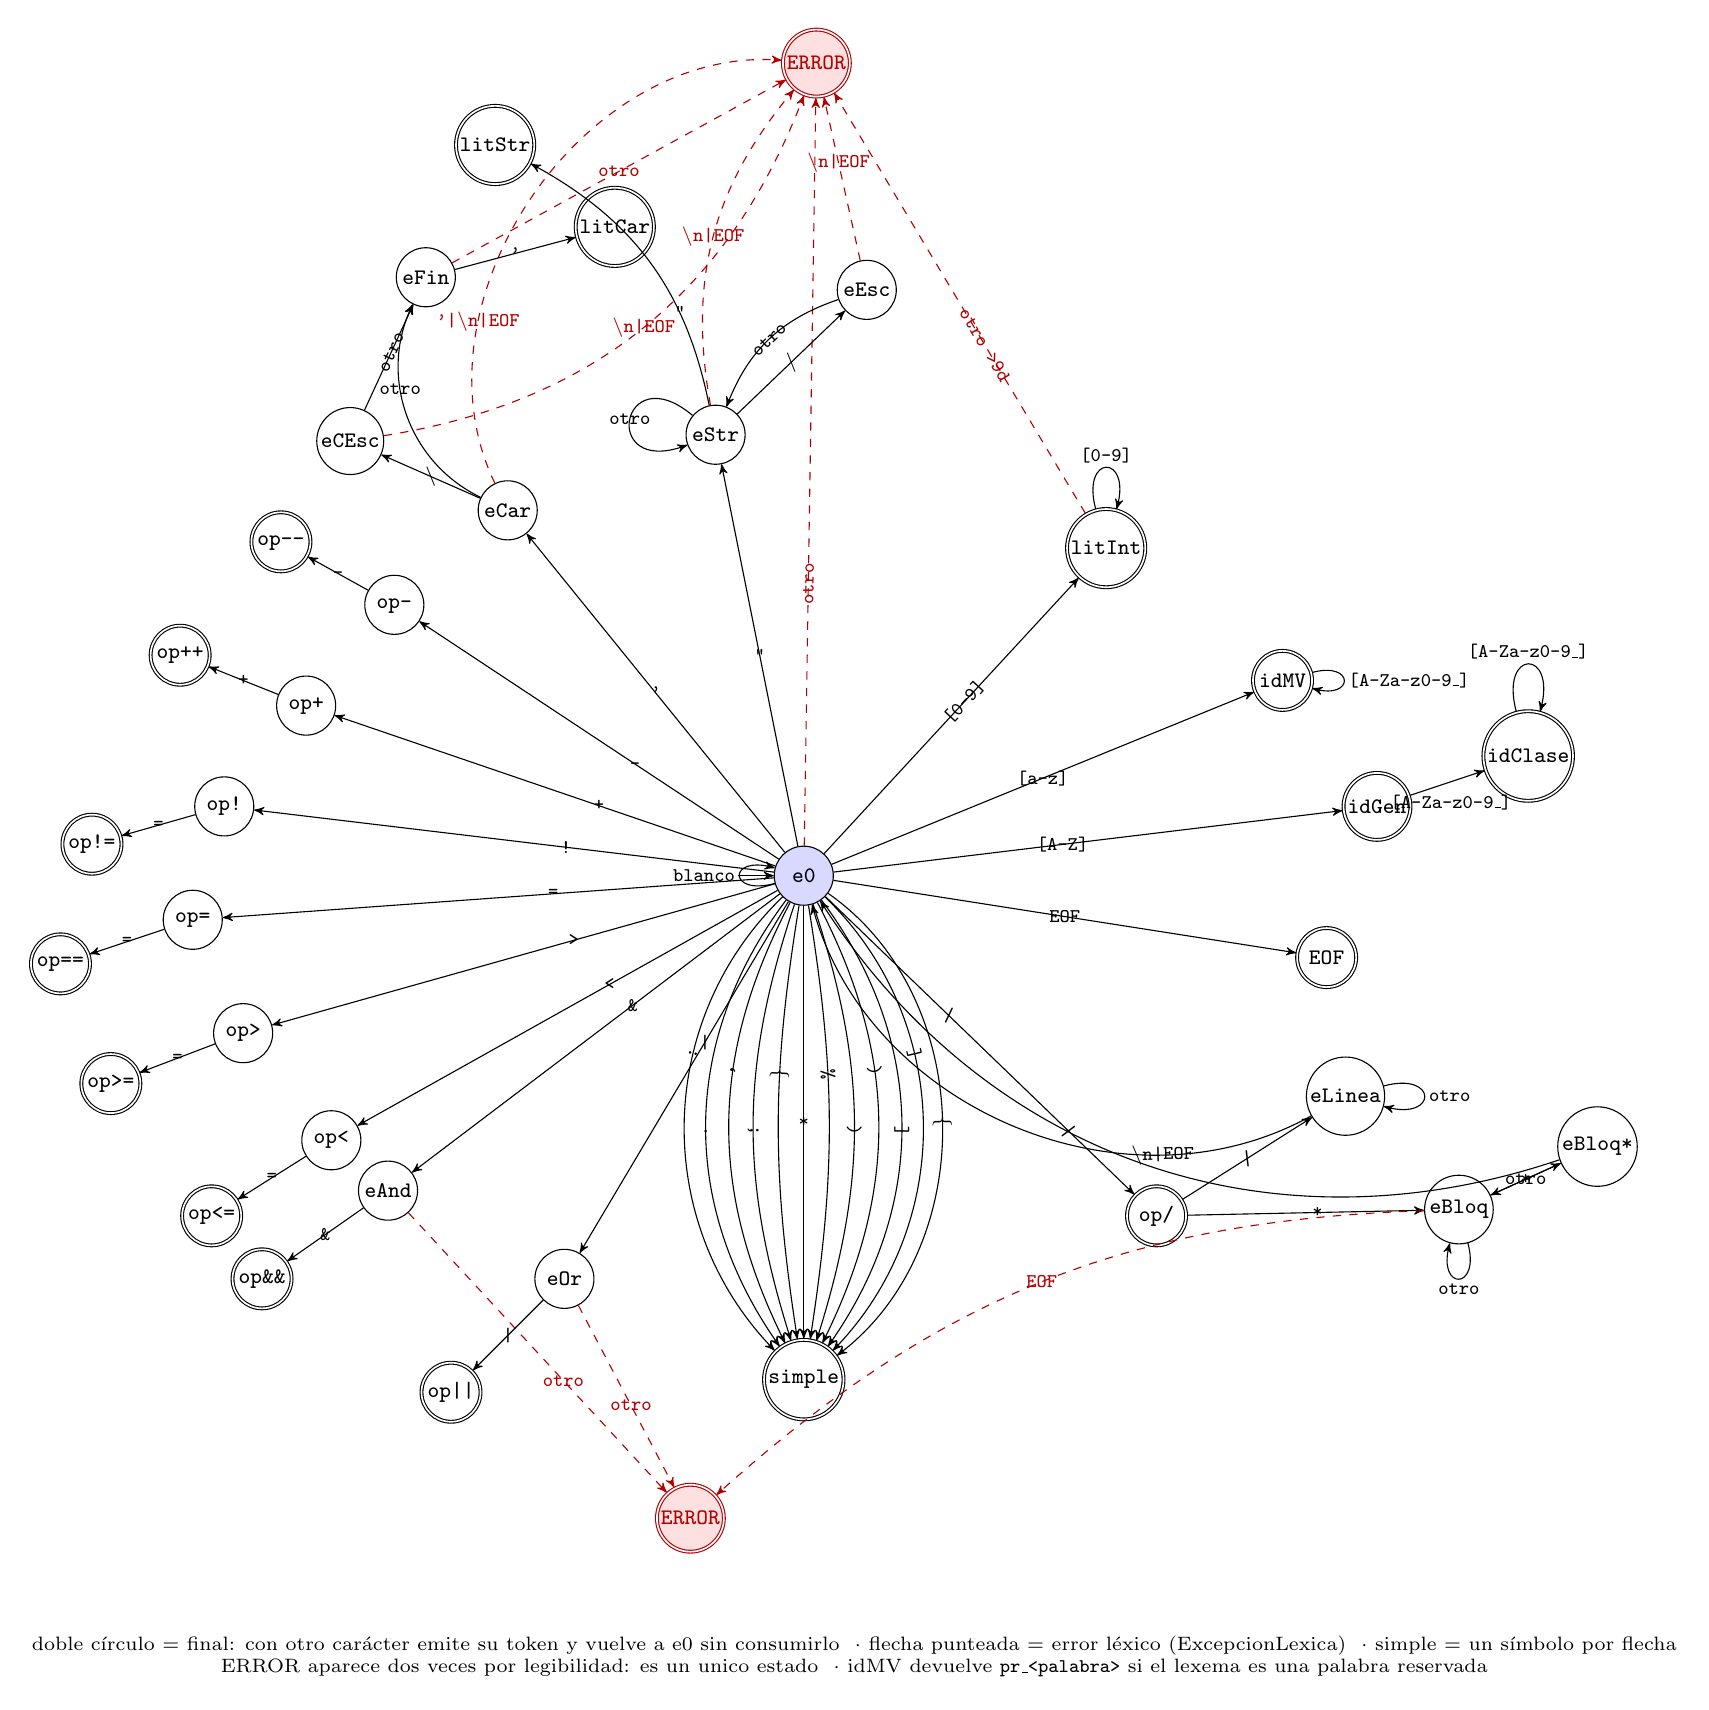
\begin{tikzpicture}[x=0.8cm, y=0.8cm, node distance=1mm]

  % ---------- e0 (centro) ----------
  \node[state, initial, initial text={}, fill=blue!15] (e0) at (0,0) {\textbf{e0}};

  % ---------- Noreste: entero e identificadores ----------
  \node[state, accepting] (ent) at (4.8,5.2) {litInt};
  \node[state, accepting] (idmv) at (7.6,3.1) {idMV};
  \node[state, accepting] (idgen) at (9.1,1.1) {idGen};
  \node[state, accepting] (idclase) at (11.5,1.9) {idClase};

  % ---------- Este-sureste: EOF y comentarios ----------
  \node[state, accepting] (eof) at (8.3,-1.3) {EOF};
  \node[state, accepting] (ediv) at (5.6,-5.4) {op/};
  \node[state] (elinea) at (8.6,-3.5) {eLinea};
  \node[state] (ebloq) at (10.4,-5.3) {eBloq};
  \node[state] (ebloqx) at (12.6,-4.3) {eBloq*};

  % ---------- Sur: simple, and/or ----------
  \node[state, accepting] (simple) at (0,-8) {simple};
  \node[state] (eor) at (-3.8,-6.4) {eOr};
  \node[state, accepting] (oor) at (-5.6,-8.2) {op||};
  \node[state] (eand) at (-6.6,-5) {eAnd};
  \node[state, accepting] (oand) at (-8.6,-6.4) {op\&\&};

  % ---------- ERROR (sur) ----------
  \node[state, accepting, fill=red!12, draw=red!70!black, text=red!70!black]
    (errs) at (-1.8,-10.2) {\textbf{ERROR}};

  % ---------- Oeste: operadores ----------
  \node[state] (emen) at (-7.5,-4.2) {op<};
  \node[state, accepting] (omen2) at (-9.4,-5.4) {op<=};
  \node[state] (emay) at (-8.9,-2.5) {op>};
  \node[state, accepting] (omay2) at (-11,-3.3) {op>=};
  \node[state] (eig) at (-9.7,-0.7) {op=};
  \node[state, accepting] (oig2) at (-11.8,-1.4) {op==};
  \node[state] (enot) at (-9.2,1.1) {op!};
  \node[state, accepting] (onot2) at (-11.3,0.5) {op!=};
  \node[state] (emas) at (-7.9,2.7) {op+};
  \node[state, accepting] (omas2) at (-9.9,3.5) {op++};
  \node[state] (emenos) at (-6.5,4.3) {op-};
  \node[state, accepting] (omenos2) at (-8.3,5.3) {op--};

  % ---------- Noroeste: literal caracter ----------
  \node[state] (ecar) at (-4.7,5.8) {eCar};
  \node[state] (ecec) at (-7.2,6.9) {eCEsc};
  \node[state] (efin) at (-6,9.5) {eFin};
  \node[state, accepting] (litcar) at (-3,10.3) {litCar};

  % ---------- Norte: literal string y ERROR (norte) ----------
  \node[state] (estr) at (-1.4,7) {eStr};
  \node[state] (eesc) at (1,9.3) {eEsc};
  \node[state, accepting] (litstr) at (-4.9,11.6) {litStr};
  \node[state, accepting, fill=red!12, draw=red!70!black, text=red!70!black]
    (errn) at (0.2,12.9) {\textbf{ERROR}};

  % ================= e0 =================
  \path
    (e0) edge[lab] node[lab, pos=0.55, sloped] {[0-9]} (ent)
    (e0) edge[lab] node[lab, pos=0.5] {[a-z]} (idmv)
    (e0) edge[lab] node[lab, pos=0.45] {[A-Z]} (idgen)
    (e0) edge[lab] node[lab, pos=0.5] {EOF} (eof)
    (e0) edge[lab] node[lab, pos=0.5] {"} (estr)
    (e0) edge[lab] node[lab, pos=0.5] {'} (ecar)
    (e0) edge[lab, loop left, looseness=8] node[lab] {blanco} (e0)
    (e0) edge[lab] node[lab, pos=0.4] {+} (emas)
    (e0) edge[lab] node[lab, pos=0.4] {-} (emenos)
    (e0) edge[lab] node[lab, pos=0.4] {=} (eig)
    (e0) edge[lab] node[lab, pos=0.4] {!} (enot)
    (e0) edge[lab] node[lab, pos=0.4] {>} (emay)
    (e0) edge[lab] node[lab, pos=0.4] {<} (emen)
    (e0) edge[lab] node[lab, pos=0.4] {\&} (eand)
    (e0) edge[lab] node[lab, pos=0.4] {|} (eor)
    (e0) edge[lab] node[lab, pos=0.4] {/} (ediv)
    (e0) edge[lab] node[lab, pos=0.5] {*} (simple)
    (e0) edge[lab, bend left=9]  node[lab, pos=0.38, sloped] {\%} (simple)
    (e0) edge[lab, bend left=18] node[lab, pos=0.52, sloped] {(} (simple)
    (e0) edge[lab, bend left=27] node[lab, pos=0.38, sloped] {)} (simple)
    (e0) edge[lab, bend left=36] node[lab, pos=0.52, sloped] {[} (simple)
    (e0) edge[lab, bend left=45] node[lab, pos=0.36, sloped] {]} (simple)
    (e0) edge[lab, bend left=54] node[lab, pos=0.5, sloped] {\{} (simple)
    (e0) edge[lab, bend right=9]  node[lab, pos=0.38, sloped] {\}} (simple)
    (e0) edge[lab, bend right=18] node[lab, pos=0.52, sloped] {;} (simple)
    (e0) edge[lab, bend right=27] node[lab, pos=0.38, sloped] {,} (simple)
    (e0) edge[lab, bend right=36] node[lab, pos=0.52, sloped] {.} (simple)
    (e0) edge[lab, bend right=45] node[lab, pos=0.36, sloped] {:} (simple)
    (e0) edge[err] node[lab, pos=0.35, sloped] {otro} (errn);

  % ================= identificadores y entero =================
  \path
    (idmv) edge[loop right, looseness=7] node[lab] {[A-Za-z0-9\_]} (idmv)
    (idgen) edge[lab] node[lab, pos=0.55, below=3pt] {[A-Za-z0-9\_]} (idclase)
    (idclase) edge[loop above, looseness=7] node[lab] {[A-Za-z0-9\_]} (idclase)
    (ent) edge[loop above, looseness=7] node[lab] {[0-9]} (ent)
    (ent) edge[err] node[lab, pos=0.4, sloped] {otro >9d} (errn);

  % ================= string =================
  \path
    (estr) edge[loop, out=140, in=200, looseness=8] node[lab] {otro} (estr)
    (estr) edge[lab] node[lab, pos=0.5] {\textbackslash} (eesc)
    (estr) edge[lab, bend right=25] node[lab, pos=0.3] {"} (litstr)
    (estr) edge[err, bend left=25] node[lab, pos=0.5] {\textbackslash n|EOF} (errn)
    (eesc) edge[lab, bend right=25] node[lab, pos=0.5, sloped] {otro} (estr)
    (eesc) edge[err] node[lab, pos=0.6] {\textbackslash n|EOF} (errn);

  % ================= caracter =================
  \path
    (ecar) edge[lab] node[lab, pos=0.5] {\textbackslash} (ecec)
    (ecar) edge[lab, bend left=45] node[lab, pos=0.62] {otro} (efin)
    (ecar) edge[err, bend left=60] node[lab, pos=0.28] {'|\textbackslash n|EOF} (errn)
    (ecec) edge[lab] node[lab, pos=0.55, sloped] {otro} (efin)
    (ecec) edge[err, bend right=30] node[lab, pos=0.5] {\textbackslash n|EOF} (errn)
    (efin) edge[lab] node[lab, pos=0.5] {'} (litcar)
    (efin) edge[err] node[lab, pos=0.5] {otro} (errn);

  % ================= operadores =================
  \path
    (emas) edge[lab] node[lab, pos=0.5] {+} (omas2)
    (emenos) edge[lab] node[lab, pos=0.5] {-} (omenos2)
    (eig) edge[lab] node[lab, pos=0.5] {=} (oig2)
    (enot) edge[lab] node[lab, pos=0.5] {=} (onot2)
    (emay) edge[lab] node[lab, pos=0.5] {=} (omay2)
    (emen) edge[lab] node[lab, pos=0.5] {=} (omen2)
    (eand) edge[lab] node[lab, pos=0.5] {\&} (oand)
    (eand) edge[err] node[lab, pos=0.6] {otro} (errs)
    (eor) edge[lab] node[lab, pos=0.5] {|} (oor)
    (eor) edge[err] node[lab, pos=0.55] {otro} (errs);

  % ================= division y comentarios =================
  \path
    (ediv) edge[lab] node[lab, pos=0.5, sloped] {/} (elinea)
    (ediv) edge[lab] node[lab, pos=0.55] {*} (ebloq)
    (elinea) edge[loop right, looseness=7] node[lab] {otro} (elinea)
    (elinea) edge[lab, bend left=52] node[lab, pos=0.25, sloped] {\textbackslash n|EOF} (e0)
    (ebloq) edge[lab] node[lab, pos=0.5] {*} (ebloqx)
    (ebloq) edge[loop below, looseness=7] node[lab] {otro} (ebloq)
    (ebloq) edge[err, bend right=20] node[lab, pos=0.5] {EOF} (errs)
    (ebloqx) edge[lab, bend left=38] node[lab, pos=0.6, sloped] {/} (e0)
    (ebloqx) edge[lab] node[lab, pos=0.5] {otro} (ebloq);

  % ---------- leyenda ----------
  \node[lg, align=center] at (0.8,-12.4)
    {doble c\'irculo = final: con otro car\'acter emite su token y vuelve a e0 sin consumirlo
     \ $\cdot$ flecha punteada = error l\'exico (ExcepcionLexica)
     \ $\cdot$ simple = un s\'imbolo por flecha\\
     ERROR aparece dos veces por legibilidad: es un unico estado
     \ $\cdot$ idMV devuelve {\ttfamily pr\_<palabra>} si el lexema es una palabra reservada};

\end{tikzpicture}
\end{center}
\end{document}
